% Chapter Template

\chapter{The Use of Semi-supervised Learning in Classification of English Grammatical Structures} % Main chapter title

\label{Chapter2} % Change X to a consecutive number; for referencing this chapter elsewhere, use \ref{ChapterX}

\section{Introduction}

The need to assess the difficulty of written texts is crucial in foreign language learning and teaching. Language instructors need a text difficulty metric that conforms to the guidelines of foreign language learning and teaching to find reading materials that match the proficiency level of their learners. Similarly, curricula designers and textbook publishers need such a metric to provide reliable and consistent learning resources and activities. Existing text evaluation metrics (\cite{kincaid1975flesch}, \cite{stenner2006accurate}, \cite{landauer2011word}, \cite{graesser2011coh}) either do not conform to educational guidelines, or they are too broad to be useful for language learning and teaching purposes. Perhaps, the most popular text evaluation tools designed for educators is ETS's TextEvaluator \citep{napolitano2015online}. It evaluates a written text based on a number of criteria that include coherence, cohesion, lexical density and syntactic difficulty. However, their syntactic difficulty feature still does not accommodate teachers' need. For example, if a teacher wants to provide their intermediate-level learners with a reading passage that features the language of cause and effect, or if-conditionals, a tool like ETS's TextEvaluator does not help much, considering the categorization features they use such as average sentence length, average number of modifiers per noun phrase, average number of dependent clauses per sentence \citep{ets_txt_eval}. Therefore, in this chapter we design and implement a system that classifies a written text into three level of grammatical difficulty, are aligned with Common European Framework Reference (CEFR) \citep{council2001common} language learning standards. 

Common European Framework Reference (CEFR) is a standard for describing language achievement on a six-point scale from A1 for beginners up to C2 for proficient users' ability on the four primary skills (reading, writing, listening, speaking) and the two secondary skills: vocabulary and grammar. The latter two skills are considered the backbone for the four primary skills in terms of difficulty. For example, a frequently uncommon lexical item like \emph{sagacious} makes the sentence in which it appears more difficult to an English learner than a sentence with a more frequent lexical item like \emph{wise}. Similarly, grammatical structures also play a vital role in the overall difficulty of a sentence. For instance, the word \emph{should} conveys a different meaning in (1) \emph{I should study for my final exams} than in (2) \emph{This is your mission should you accept it}. The latter is considered more difficult to an English learner because the use of should as a conditional is less frequent than its use as a modal auxiliary expressing necessity according to CEFR \citep{council2001common}. 

The English Grammar Profile (EGP) \citep{o2017english} is a finite list of (1222) grammar features compiled from the Cambridge Learner Corpus, which comprises over 250,000 scripts from Cambridge English Exams at all levels. The purpose of EGP is to establish which grammatical features characterizes learners' output at each level of CEFR. \citep{o2017english} The list contains structural features, their corresponding CEFR levels and example sentences \ref{tab:cefr}

Our goal in this chapter is to train a multinomial logistic regression classifier on the example sentences derived from EPG to predict the CEFR difficulty level. Due to the limited number of examples sentences (around 3000), we combine each two levels (e.g. A1,A2) into one class (A), so we end up with three super-levels: A, B, and C , which correspond to  elementary, intermediate, and advanced levels, respectively. We also improve the performance of the classification by applying a bootstrapping technique \citep{yarowsky_unsupervised_1995} to fetch data from external sources to supplement the training data. Finally, we evaluate the performance of the classification before and after the bootstrapping against a random classifier.

%In this chapter, we examine the use of multinomial logistic regression classifier in a semi-supervised manner to automatically categorize English sentences based on difficulty to second language learners using the Common European Framework Reference. We also compare some of text representation techniques introduced in the previous chapter and determine the best one to use in this task. Finally, we evaluate the overall performance of the classifier before and the semi-supervised data augmentation. 
%
%Common European Framework Reference (CERF) is a standard for describing language achievement on a six-point scale, from A1 for beginners, up to C2 for proficient user ability on the four primary skills reading, writing, listening, speaking, and the two secondary skills: vocabulary and grammar. The latter two skills are considered the backbone for the four primary skills in terms of difficulty. For example, a frequently uncommon lexical item like \emph{sagacious} makes the sentence in which it appears more difficult to an English learner than a sentence with a more frequent lexical item like \emph{wise}. Similarly, grammatical structures also play a vital role in the overall difficulty of a sentence. For instance, the word \emph{should} conveys a different meaning in \emph{I should study for my final exams.} than in \emph{This is your mission should you accept it.}. The latter is considered more difficult to an English learner because the use of \emph{should} as a conditional is less frequent than its use as a modal auxiliary expressing necessity. 
%
%Wide World Web and social media are becoming indispensable resources for second language learners. However, deciding the appropriateness of materials to learners is a very labor-intensive task for English teachers. Instructors spent hours sifting through materials online to determine their difficulty and whether or not they are appropriate for their learners. To this end, we leverage the power of machine learning to build a tool that can automatically determine the difficulty of a given text according to CEFR guidelines. 
%CEFR provides 1200 criteria \citep{noauthor_english_nodate} for the difficutly of grammatical structures \ref{tab:cefr}.
%\begin{table}
%\caption{An excerpt of English sentences and their corresponding CEFR difficulty levels}
%\centering
%\begin{tabular}{l|c|c|c}
%Sentence   & Level \\
%\hline
%I go there every year with my friends & A1 & \\
%I think swimming is good for my body. & A2 & \\
%Tomorrow I'm expecting a delivery of our latest\\ catalogues. & B1 & \\
%Do not hesitate to contact me should \\you need further information. & B2 & \\
%Living in Greece, I have had a chance \\to realise how much tourism can affect one's life. & C1 & \\
%There were no photographs of \\him in Ann 's mother's albums. & C2 & \\
%\end{tabular}
%\label{tab:cefr}
%\end{table}

\begin{table}
\centering

\caption{Example of CEFR Grammatical Rules}
\resizebox{\textwidth}{!}{\begin{tabular}{|l|l|l|l|} 
\hline
Level & guideword                                                                                  & Can-do statement                                                                                                                                                                                        & \multicolumn{1}{l|}{Example}                                                                                                                                                                              \\ 
\hline
A1    & \begin{tabular}[c]{@{}l@{}}FORM: COMBINING TWO \\ADJECTIVES WITH 'AND'\end{tabular}        & \begin{tabular}[c]{@{}l@{}}Can use 'and' to join a limited\\~range of common adjectives.~\end{tabular}                                                                                                  & The teachers are very nice and friendly.                                                                                                                                                                  \\ 
\hline
A2    & \begin{tabular}[c]{@{}l@{}}FORM: COMBINING TWO \\ADJECTIVES WITH 'BUT'\end{tabular}        & \begin{tabular}[c]{@{}l@{}}Can use 'but' to join a limited range \\of common adjectives, after 'be'.\end{tabular}                                                                                       & The weather was cloudy but fine.                                                                                                                                                                          \\ 
\hline
B1    & \begin{tabular}[c]{@{}l@{}}FORM/USE: \\'THE' + NOUN + 'WHO/THAT', FOCUS\end{tabular}       & \begin{tabular}[c]{@{}l@{}}Can use defining relative clauses, \\'the person who/that, the thing that, \\the (only) one who/that' as a focusing device.~\end{tabular}                                    & \begin{tabular}[c]{@{}l@{}}The thing that was great is that the \\weather was really warm and it didn't rain.~\end{tabular}                                                                               \\ 
\hline
B2    & FORM/USE: 'LET'S NOT', SUGGESTION                                                          & \begin{tabular}[c]{@{}l@{}}Can use 'let's not' + base form of \\a main verb to make a suggestion.~\end{tabular}                                                                                         & Let's not lose track of each other again!                                                                                                                                                                 \\ 
\hline
C1    & \begin{tabular}[c]{@{}l@{}}FORM/USE:\\~'NOT ONLY … BUT ALSO'\\~WITH INVERSION\end{tabular} & \begin{tabular}[c]{@{}l@{}}Can use inverted auxiliary \\'do' + the subject after 'not only', t\\o give focus.\end{tabular}                                                                              & \begin{tabular}[c]{@{}l@{}}Indeed, not only did they teach us useful knowledge, \\but they also organised practical exercises to ensure\\~that we had assimilated all the information.\end{tabular}       \\ 
\hline
C2    & FORM/USE: 'NEITHER'                                                                        & \begin{tabular}[c]{@{}l@{}}Can use 'Neither' or 'Nor' + inverted auxiliary or 'be' \\+ subject to add to a previous related negative clause, \\to focus on an additional negative factor.~\end{tabular} & \begin{tabular}[c]{@{}l@{}}Maybe he will eventually get over this terrible experience, \\but he's bound to be a lonelier boy than he was. \\Nor does Jack's future look any more promising.\end{tabular}  \\
\hline
\end{tabular}}
\label{tab:cefr}

\end{table}

%We treat this task as a multinomial classification problem. In our first attempt, we train a logistic regression classifier optimized by Newton-Raphson method on a dataset of around 3000 examples provided by [englishprofile.com], described in details in section 2. We get an F1 score of 0.67. In our second attempt, we use the trained classifier from our first attempt to predict the difficulty of sentences in an unlabeled corpus to fetch more training. After that, we merge the newly fetched data with the original dataset (obtained from Englishprofile.com) and re-train another multinomial logistic regression classifier from scratch to get an F1 score of 0.79. 

\section{Related Works}
\label{sec:research_background}

Sentence classification is the most common task in natural language processing. A considerable number of studies \citep{liu2012survey, pang2002thumbs, stamatatos2009survey} have been conducted on lexicalized tasks like sentiment analysis, spam filtering, news categorization, etc. Rarely do we see work on classification sentences based on their syntactic structures. Thus, to the best of our knowledge, no work has ever tackled the task of classifying the grammatical difficulty of English sentences according to CEFR guidelines. Therefore, we will briefly survey techniques used to solve general sentence classification problems. 

Proximity-based Algorithms such as Rocchio's algorithm \citep{rocchio1971relevance}  and K-nearest neighbor \citep{tam_comparative_2002} built vectors for each class using a training set of a document by measuring the similarity, such as Euclidean distance or cosine similarity, between the documents. Some studies \citep{bang_hierarchical_2006} incorporated dictionary-based methods to construct a conceptual similarity with KNN classifier, while \citep{chang_using_2009} combined two KNN classifier with a Naive Bayes one using TF-IDF over phrases to categorize large collections of emails. While proximity-based methods perform well on document classification, yet using them on a large training set is not feasible, for computing similarities across documents is computationally and resource-wise expensive. Another disadvantage is that noise, and irrelevant data can severely degrade classification performance.

Another family of classifiers that work well in text category tasks is decision trees. Classification using this method is done via automatically creating  "if-then" rules. Their use in tasks like spam filtering is widespread even with the advent of deep neural network methods \citep{wu_behavior-based_2009}. Another common powerful classifier is Naive Bayes that based on Bayes' rule, which performs surprisingly well for many real-world classification applications under some specific conditions \citep{mccallum1998comparison, rish_analysis_2001}. While Naive Bayes does not often outperform discriminative classifiers like Support-Vector Machine, it has the advantage of functioning well with small training data. \citep{kim_effective_2006} and \citep{isa_text_2008} showed promising results by selecting Naive Bayes with SVM for text classification and clustering the documents. Using a Poisson Naive Bayes for text classification model also yielded excellent results \citep{isa_text_2008}.  
 
The SVM classification method and logistic regression have shown outstanding results when used in text classification tasks \citep{Yang1999ARO} \citep{brucher2002document} perhaps because of their capacity of handling high-dimensional sparse data well.  However, they can be relatively complex in training and require lengthy time and resource consumption.



\section{Methods}
\label{sec:logistic}

\subsection{Dataset: English Grammar Profile}
The dataset used for this study, provided by English Grammar Profile, exhibits a typical grammar profile for each level. It consists of 3615 examples and 1215 rules \ref{tab:cefr}, divided as follows: class A has 1194 supporting examples; class B has 1775 examples, and class C has 646 supporting examples. We merged the six levels into three supercategories in order to provide more data within each category. 

The dataset provides some guidance of what characterizes each example. These rules are prepared to be used by ESL teachers, and they are not very computationally friendly. For example, one rule of indicating the membership of a sentence into A2 class is having "a non-defining relative clause with 'which' as the subject". A trained English teacher can easily spot a sentence with such a rule, yet detecting it using regular expression, for instance, is very difficult to achieve. On the other hand, the small number of examples in the dataset is not enough to build a reliable probabilistic classifier to learn to distinguish the various properties of the classes. Therefore, in order to improve the performance, we utilize a semi-supervised data augmentation technique similar to Yarawsky's bootstrapping approach \citep{yarowsky_unsupervised_1995}. 

\begin{figure}[t]
    \centering
    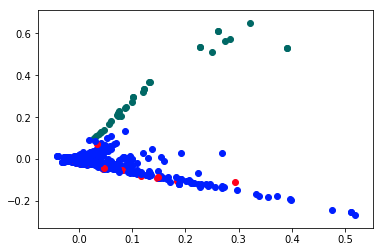
\includegraphics[width=.75\linewidth]{../Figures/pca_proj.png} 
    \caption{Two Dimensional Projection of classes A, B and C using K-means Clustering and Principal Component Analysis}
    \label{fig:kmeans_pca}
\end{figure}

\subsection{Multinomial Logistic Regression}
Suppose that $\mathbf{x}$ is the vectorized sentence in either of its two forms: BOW or TF-IDF, $y\in Y$ is the class label, and $\mathbf{w}_k$ and $b_k$ are network parameters associated with class $y$. Then the probability of $\mathbf{x}$ belonging to the class $y$ can be defined by the Softmax function:
\begin{equation}
p(y|\mathbf{x}) =\frac{1}{z(\mathbf{x})}\exp(\mathbf{w}_y^T\mathbf{x}+b_y) \,,
\label{eq:softmax}
\end{equation}
where $z(\mathbf{x}) = \sum_{j=1}^{K}\exp(\mathbf{w}_j^T\mathbf{x}+b_j)$.

Let the log-likelihood function be $$L ( \beta ) = \sum _ { i = 1 } ^ { N } \log p _ { g _ { i } } \left( x _ { i } ; \beta \right)$$. 

$$= \sum _ { i = 1 } ^ { N } \left[ \overline { \beta } _ { g _ { i } } ^ { T } x _ { i } - \log \left( 1 + \sum _ { l = 1 } ^ { K - 1 } e ^ { \overline { \beta } _ { l } ^ { T } x _ { i } } \right) \right]$$

To apply the Newton-Raphson method, we need the second derivative of the log-likelihood function

$$\frac { \partial ^ { 2 } L ( \beta ) } { \partial \beta _ { k j } \partial \beta _ { m n } } = - \sum _ { i = 1 } ^ { N } x _ { i j } x _ { i n } p _ { k } \left( x _ { i } ; \beta \right) \left[ l ( k = m ) - p _ { m } \left( x _ { i } ; \beta \right) \right]$$

The formula for updating $\beta_{new}$ for multiclass is:
$$\beta ^ { \text { new } } = \beta ^ { \text { old } } + \left( \tilde { \mathbf { X } } ^ { T } \mathbf { W } \tilde { \mathbf { X } } \right) ^ { - 1 } \tilde { \mathbf { X } } ^ { T } ( \mathbf { y } - \mathbf { p } )$$

where $y$ is the concatenated indicator vector of dimension $N \times (K-1)$, $p$ is the concatenated vector of fitted probabilities of dimension $N \times (K-1)$, $\tilde{X}$ is an $N(K-1)\times (p+1)(K-1)$ matrix; and Matrix $W$ is an $N(K-1)\times N(K-1)$ square matrix. \citep{friedman2001elements}

\subsection{Feature Design}

For this task, we are comparing two standard methods of feature generation in natural language processing and information retrieval: Bag-of-Words model and term-frequency inverse-document frequency (TF-IDF)

%\subsubsection{Bag of Word Model} a method to represent the occurrence of words within one sentence. We add different variation by counting unigram, bigram and trigram frequencies. Besides, because this model ignores the order or the location of the word in the sentence, it might not be that helpful to our task as it is not lexicalized and the grammar is the core of it. Therefore, we replace noun and adjective words with their parts-of-speech tags in order to enforce the presence of the grammatical category and avoid the influence of the word itself.  For example, the sentence "this is your mission should you accept it” becomes this is NP should S-PRN VRB O-PRN (CLAUSE)”. 
%
%\subsubsection{TF-IDF}  This common information retrieval technique differs from the regular bag-of-words model in that length of the sentence, and the frequency of words across sentences does not influence the score of a sentence as it is normalized by other sentences in the dataset. TF·IDF is calculated based on term frequency and document frequency. Term frequency is the number of times a term $t$ occurs in a document $d$ , denoted by TF (t, d) . Document frequency measures the number
%of documents in which a term t occurs, denoted by DF(t) . TF·IDF is typically calculated as:
%
%$$T F \cdot I D F ( t , d ) = T F ( t , d ) \cdot \log \frac { | D | } { D F ( t ) }$$, where $|D|$ is the total number of documents.





\section{Experimental Results}
\label{sec:exp}

In this section, we evaluate several variations of our method against a random model as our baseline model. In the following experiments, all methods are conducted using Python 3.5 and Scikit Learn Library tested on MacBook Pro laptop with Core i5 processor and 8 GB of RAM.

\subsection{First Phase}

In the first phase of our experiment, we train a logistic regression classifier, optimized by the Newton-Raphson method, on the English Grammar Profile dataset. We also introduce a  feature design method to mask word categories with their part-of-speech tags in order to preserve grammatical information and avoid the lexical influence of the word. We refer to this method as \emph{Masked} in Table \ref{tb:egp_lr_performance}. We use a combination of feature design methods such as:

\begin{itemize}
    \item \textbf{BOW}: Apply unigram, bigram and trigram Bag-of-Words model with both word tokens, and masked tokens.
    \item \textbf{TF-IDF}: Apply unigram, bigram and trigram TF-IDF model with both word tokens, and masked tokens.
\end{itemize}


\begin{figure}[t]
    \centering
    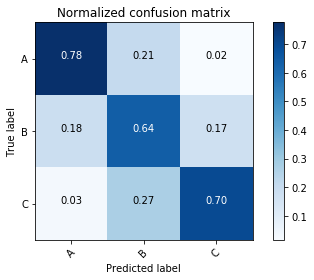
\includegraphics[width=.75\linewidth]{../Figures/conf_matrix_iter1.png} 
    \caption{Confusion matrix illustrating the performance of LR-BOW-Word model with class weight to deal with data imbalance}
    \label{fig:egp_confmat_LRBOW}
\end{figure}

\begin{table}
\centering
\caption{Comparison of Logistic Regression Performance Using Multiple Feature Extraction Methods}
\begin{tabular}{|l|c|c|c|} 
\hline
Model                  & Precision \%    & Recall \%       & F1 \%            \\ 
\hline
Random-Baseline        & 39 \%           & 39 \%           & 39 \%            \\ 
\hline
\textbf{BOW-LR-Words}  & 70 \%           & \textbf{69} \%  & \textbf{69} \%   \\ 
\hline
BOW-LR-Masked          & 66 \%           & 62 \%           & 63 \%            \\ 
\hline
TF-IDF-LR-Words        & \textbf{75} \%  & 66 \%           & 60 \%            \\ 
\hline
TF-IDF-LR-Masked       & 66 \%           & 64 \%           & 61 \%            \\
\hline
\end{tabular}
\label{tb:egp_lr_performance}
\end{table}

From Table \ref{tb:egp_lr_performance}, we compare the performance of four variations of our method against the baseline, which is a random model. Surprisingly, we notice that our Bag-of-Words model with word tokens (BOW-LR-Words) outperform the one with the masked sequence (BOW-LR-Masked) in terms of precision and recall respectively. Besides, BOW-LR-Words also outperforms (TF-IDF-LR-Words) model in terms of recall only, while the latter has higher recall. From the confusion matrix (Fig. \ref{fig:egp_confmat_LRBOW}), we see that (BOW-LR-Words) model predicts most of the testing data correctly even though the number of training data is not equal among the classes, especially for class C. Therefore, we needed to assign specific weights to each class during the training in order to avoid this imbalance in the data. 

\subsection{Second Phase}

The results shown in Table \ref{tb:egp_lr_performance} does indicate that the linear model has learned the associations between sentences and their corresponding grammatical class reasonably well. However, both of our feature design techniques, namely BOW and TF-IDF have their disadvantages. The first assigns similarity based on occurrence, size and mutual words. For example, the BOW model learns that longer sentences tend to be the most difficult, while shorter ones are less difficult. Similarly, while TF-IDF treats the drawbacks of BOW model, it still ignores the usefulness of what-so-called \textit{Stop Words} due to their commonality. In other words, it is very hard to trust these results with this amount of training data. Therefore, we propose a non-synthetic data augmentation method to provide more training examples, and thereby improve the overall performance of the model. 

Using a text-only small version of the Brown Corpus \citep{francis1965standard}, we use our BOW-LR-Words model to predict the grammatical difficulty labels of its sentences. Next, we collect the sentences predicted with high certainty (above 0.9 probability) to be fed into the original dataset. It is crucial to set a higher probability threshold, for the new data examples will serve as seed points for our prediction in the future; we do not want the classifier to \textit{drift} from the original trajectory. \citep{curran2007minimising} This technique is reminiscent of Yarawsky's Bootstrapping \citep{yarowsky_unsupervised_1995}(semi-supervised) algorithm, but with one difference is that unlike in Yarawsky's method, we apply this step only once. 

Out of 38,400 sentences in the unlabeled corpus, only 1,428 sentences were detected with certainty above 90\%. We also removed any sentence that is longer than 30 words in order to lessen the undesirable effect of BOW technique. We apply our best model from phase one to the augmented dataset of 5,043 examples under the same training conditions to get a precision of \textbf{0.80}, a recall of \textbf{0.79}, and an F1 score of \textbf{0.79}. 

Comparing the confusion matrices before \ref{fig:egp_confmat_LRBOW} and after \ref{fig:egp_confmat_LRBOW_aug} Bootstrapping, we notice that the performance of classification to class A does not improve much, unlike in classes B and C whose classification performance increases by F1 scores of 0.10 and 0.13 respectively. 

\begin{figure}[t]
    \centering
    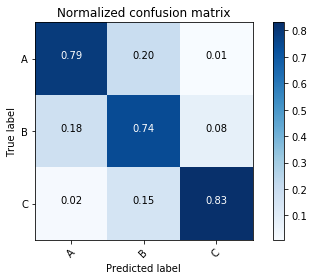
\includegraphics[width=.75\linewidth]{../Figures/conf_matrix_iter2.png} 
    \caption{Confusion Matrix Illustrating the Performance of LR-BOW-Word Model after Augmentation}
    \label{fig:egp_confmat_LRBOW_aug}
\end{figure}

\section {Conclusion}
\label{sec:conclusion}
In this chapter, we have presented a classification method based on simple multinomial logistic regression and Bag-of-Words model augmented with semi-supervised (Bootstrapping) method to classify English sentences based on their level difficulty level, A=Beginner, B=intermediate, and C=Advanced according to CEFR. We have also compared several common feature design techniques to encode the sentences along with a proposed masking BOW method that replaces lexical items with their grammatical category. Finally, the model achieves an overall F1 score of 0.69, and 0.79 after augmenting it with example sentences from an unlabeled corpus.
